\section{Theoretical Analysis}
\label{sec:analysis}

In this section we will explain with some detail how do we analyse the circuit theoretically. To do so, and because there were several things to be analyse, the following subsections are going to detail the analysis of each of the six powerpoint points related to the theoretical analysis. Just as a final note, the results obtained theoretically will only be shown in the symulation section, to compare the both.

\subsection{Point 1: Determine the initial state of the circuit}

Initially, the circuits's independent voltage source inputs in the circuit a constant voltage. Because of this, and considering that the circuit is working for a really long time (started working for t = $-\infty$), we can assume that the capacitor is already fully charged and, consequentaly, it behaves like an open circuit. So to analyse the circuit's initial state we just need to do a node analysis just like we did in \textit{laboratory nº1}. 

After performing the node analysis we've obtained the following matrix:

$\begin{pmatrix}
1 & 0 & 0 & -1 & 0 & 0 & 0 & 0\\
-G1 & G1+G2+G3 & -G2 & 0 & -G3 & 0 & 0 & 0\\
0 & -G2-Kb & G2 & 0 & Kb & 0 & 0 & 0 \\
G1 & -G1 & 0 & G4+G6 & -G4 & 0 & -G6 & 0\\
0 & 0 & 0 & -Kd*G6 & 1 & 0 & Kd*G6 & 0 \\
0 & Kb & 0 & 0 & -G5-Kb & G5 & 0 & 0 \\
0 & 0 & 0 & -G6 & 0 & 0 & G6+G7 & 0  \\ 
0 & 0 & 0 & 1 & 0 & 0 & 0 & 0
\end{pmatrix}$
$\begin{pmatrix}
V1\\
V2\\
V3\\
V4\\
V5\\
V6\\
V7\\
V8
\end{pmatrix}$
=
$\begin{pmatrix}
V5\\
0\\
0\\
0\\
0\\
0\\
0\\
0
\end{pmatrix}$

\subsection{Point 2: Determine the equivalent resistance seen by the capacitor}

To determine the equivalent resistance, we've defined a voltage source Vx between the nodes 6 and 8 and we've powered off the independent voltage source Vs. After that, we use the node analysis to determine the volatge in all nodes, which resulted in the following matrix:

$\begin{pmatrix}
0 & 0 & 0 & 0 & 0 & 1 & 0 & -1\\
-G1 & G1+G2+G3 & -G2 & 0 & -G3 & 0 & 0 & 0\\
0 & -G2-Kb & G2 & 0 & Kb & 0 & 0 & 0 \\
G1 & -G1 & 0 & G4+G6 & -G4 & 0 & -G6 & 0\\
0 & 0 & 0 & -Kd*G6 & 1 & 0 & Kd*G6 & 0 \\
1 & 0 & 0 & -1 & 0 & 0 & 0 & 0\\
0 & 0 & 0 & -G6 & 0 & 0 & G6+G7 & -G7  \\ 
0 & 0 & 0 & 1 & 0 & 0 & 0 & 0
\end{pmatrix}$
$\begin{pmatrix}
V1\\
V2\\
V3\\
V4\\
V5\\
V6\\
V7\\
V8
\end{pmatrix}$
=
$\begin{pmatrix}
Vx\\
0\\
0\\
0\\
0\\
0\\
0\\
0
\end{pmatrix}$

After knowing these voltages, it's easy to determine the currents in all branches. To determine the equivalent resistance we need to determine the current in the branch 6-8, Ix, just because $R_{eq}=V_{x}/I_{x}$. We've obtained Ix by analysing the node 8 and we've obtained the following expression for Ix:

\begin{equation}
I_x = -Kb*(V_2 - V_5) + G_5*(V_5 - V_6) 
\end{equation}

After knowing Ix, we now can obtain Req, using the previous shown formula.

\subsection{Point 3: Obtaining the natural solution for the capacitor}

Using the results in point 2, we can determine the natural solution of the circuit by making a simple RC circuit, with the only components being the capacitor and the equivalent resistance, just as shown in the figure:

\begin{figure}[H]
\centering
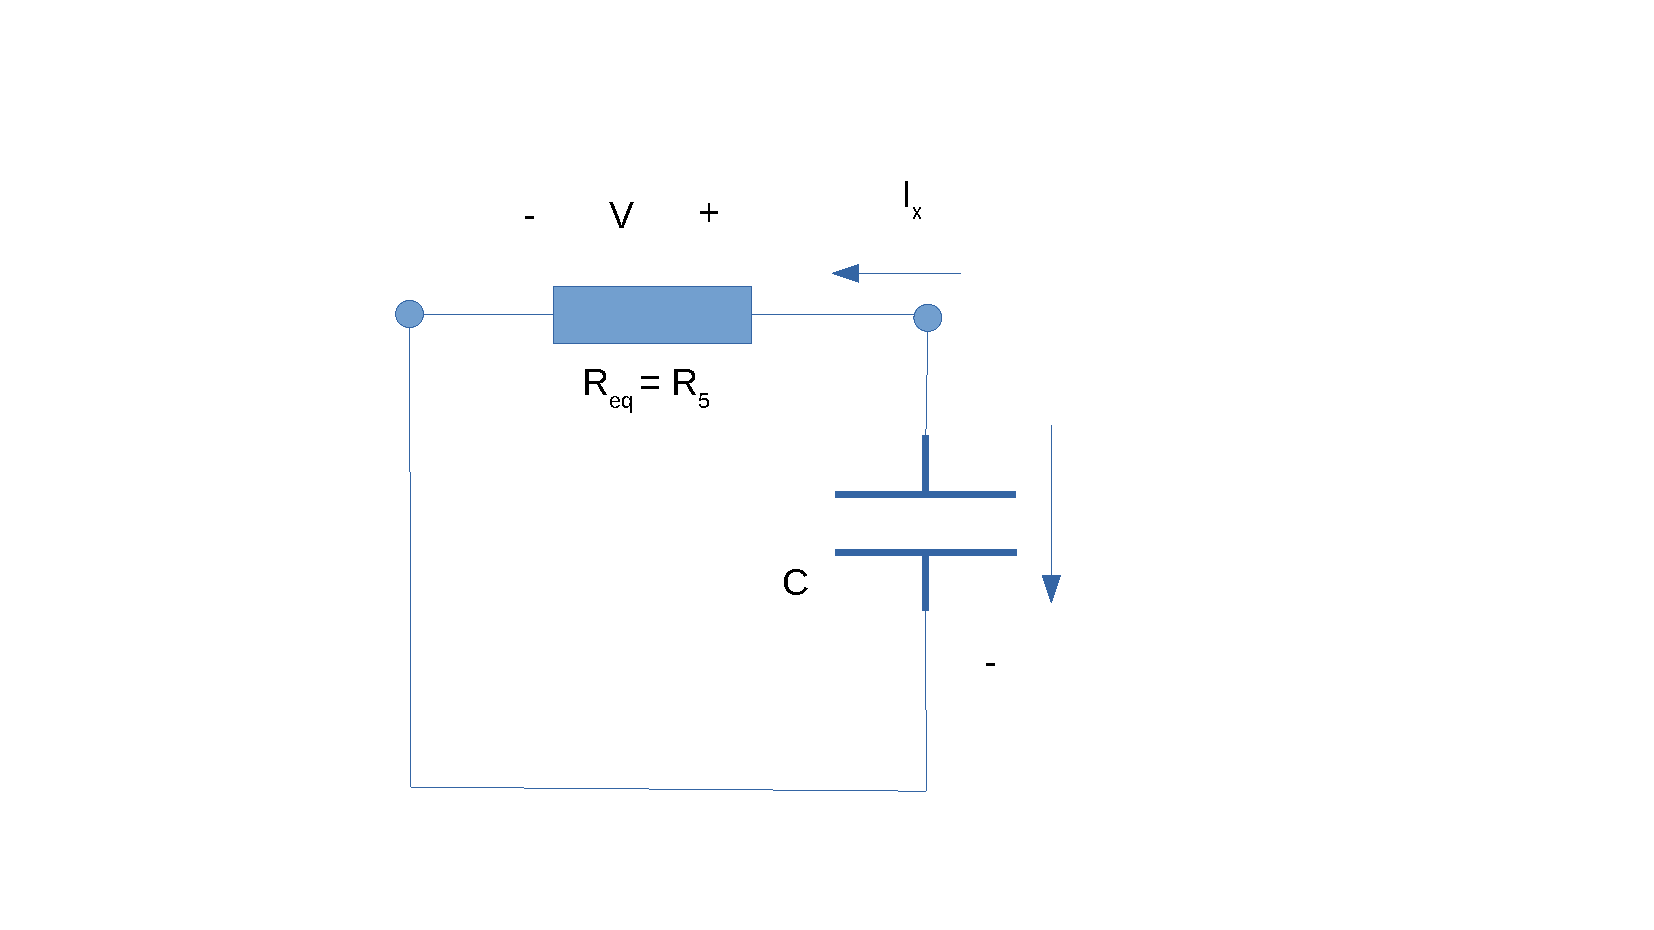
\includegraphics[width = 15cm]{circuit3.pdf}
\caption {Circuit3}
\end{figure}

Using the Kirchhoff's voltage law for this circuit, we've obtain the folling diferential equation:

\begin{equation}
\frac{dV}{dt} + \frac{V}{C*R_{eq}} = 0
\end{equation}

Knowing that the $V_{capacitor_i} = V_{6} - V_{8}$ and using the values for these voltages obtained in point 1, the natural solution for the capacitor is given by:

\begin{equation}
V_{6n} = V_{capacitor_i} * e^{-\frac{t}{C*R_{eq}}}
\end{equation}

\begin{figure}[H]
\centering
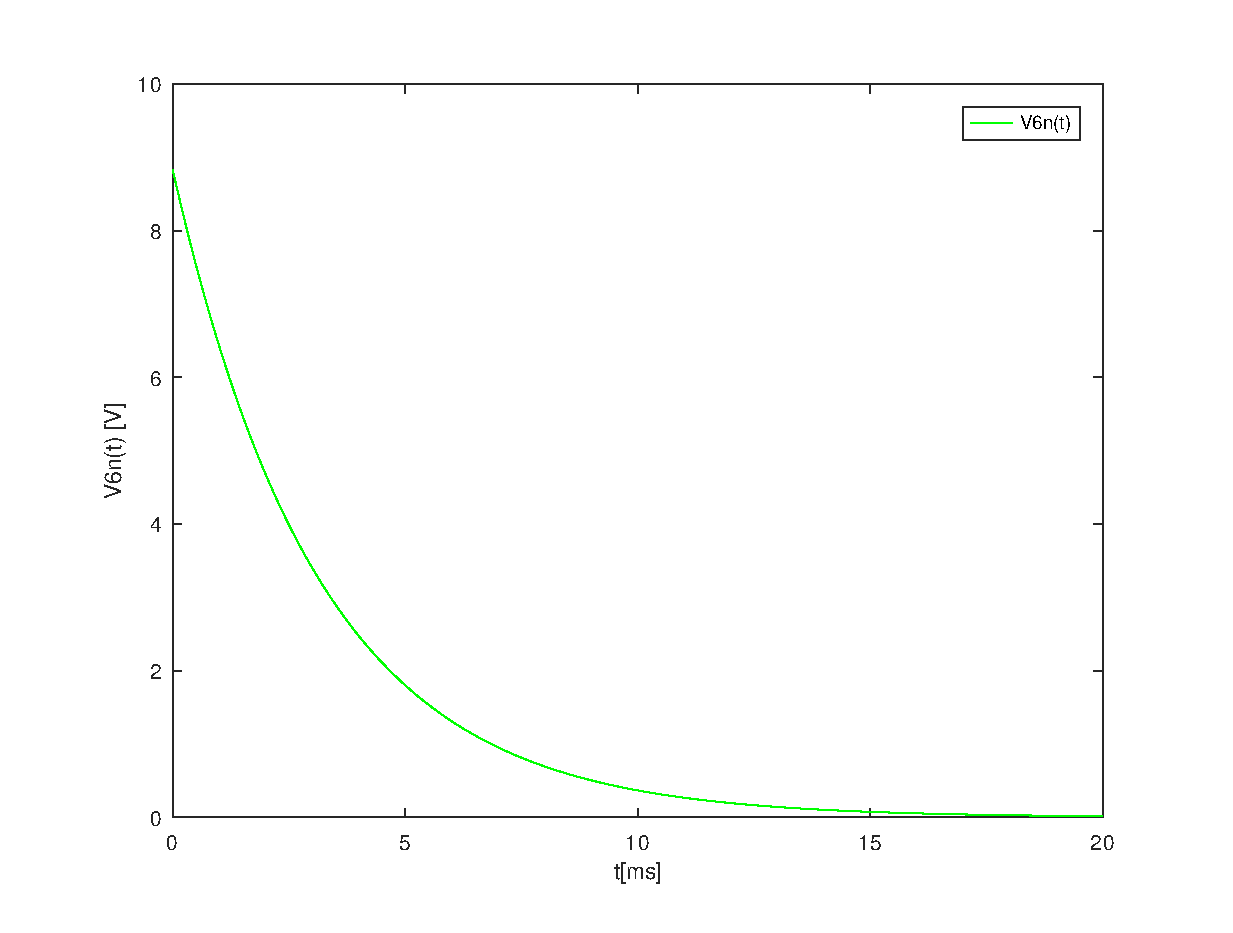
\includegraphics[width = 8cm]{NaturalResponse.eps}
\caption {Natural Response}
\end{figure}



\subsection{Point 4: Determine the forced solution for the circuit}

We already know that in a forced circuit the voltages in all nodes will gain the same frequency as the source. Knowing this we know that the solution for the node i will be $V_{i} = V_{i_{max}}*cos(w*t + \phi_{i})$. So, in order to determine the voltages for all nodes, we just need to determine the voltages amplitudes and phases, or in other words, their complex amplitude. This brings an interesting point: if we consider the complex world the solutions will be in the form of $V_{i} = V_{i_{max}}*e^{w*t} * e^{\phi_{i}}$, which makes easy to obtain both the amplitudes and the phases.
Alongside this, we just need to solve the node analysis for all the circuit, which will result in the following matrix:

$\begin{pmatrix}
1 & 0 & 0 & -1 & 0 & 0 & 0 & 0\\
-G1 & G1+G2+G3 & -G2 & 0 & -G3 & 0 & 0 & 0\\
0 & -G2-Kb & G2 & 0 & Kb & 0 & 0 & 0 \\
G1 & -G1 & 0 & G4+G6 & -G4 & 0 & -G6 & 0\\
0 & 0 & 0 & -Kd*G6 & 1 & 0 & Kd*G6 & -1 \\
0 & Kb & 0 & 0 & -G5-Kb & G5+\frac{1}{Z_c} & 0 & -\frac{1}{Z_c} \\
0 & 0 & 0 & -G6 & 0 & 0 & G6+G7 & -G7  \\ 
0 & 0 & 0 & 1 & 0 & 0 & 0 & 0
\end{pmatrix}$
$\begin{pmatrix}
V1\\
V2\\
V3\\
V4\\
V5\\
V6\\
V7\\
V8
\end{pmatrix}$
=
$\begin{pmatrix}
V_s\\
0\\
0\\
0\\
0\\
0\\
0\\
0
\end{pmatrix}$

Note: For the node 6 we have the following equation:

%equação no 6

And this is what we see in the matrix

Solving the matrix using the given values, the complex amplitudes generated are the following:

\begin{table}[H] \centering
\begin{tabular}{|
>{\columncolor[HTML]{FFCC67}}l |c|}
\hline
\multicolumn{2}{|l|}{\cellcolor[HTML]{EABD8B}Octave - Voltages (V)} \\ \hline
V1 & 1.000000e+00 + i(-1.549812e-33) V\\ \hline
V2 & 9.469010e-01 + i(-1.466518e-17) V\\ \hline
V3 & 8.361543e-01 + i(5.184518e-16) V\\ \hline
V4 & 0.000000e+00 + i(-1.549812e-33) V\\ \hline
V5 & 9.545144e-01 + i(-5.131501e-17) V\\ \hline
V6 & -5.667484e-01 + i(-8.549146e-02) V\\ \hline
V7 & -3.836423e-01 + i(2.062473e-17) V\\ \hline
V8 & -5.710758e-01 + i(3.070122e-17) V\\ \hline

\end{tabular}
\caption{Complex Amplitudes - Octave Results}
\end{table}


\subsection{Point 5: Determine the solution for the voltage in node 6}

%\[
 %V_{6}(t)=
  %  \begin{cases}
   %   V_{6i} & \text{para t $\in$ [-5, 0]}\\
   %   V_{6n}(t) + V_{6f}(t) = V_{6i}e^{$\frac{t}{C*R_5}$} + Acos($\omega$ t - $\phi$_1)
   % \end{cases}       
%\]

Using the data obtained in the points 3 and 4 is relatively easy to find the solution for the voltage in the node 6. We just need to find the forced solution using the amplitude and phase for the node 6 obtained in point 4 e aplying it in this formula: $V_{6f} = V_{6_{max}}*cos(w*t + \phi_{6})$. After that it's just add it to the natural solution and we've obtained the following:

\begin{figure}[H]
\centering
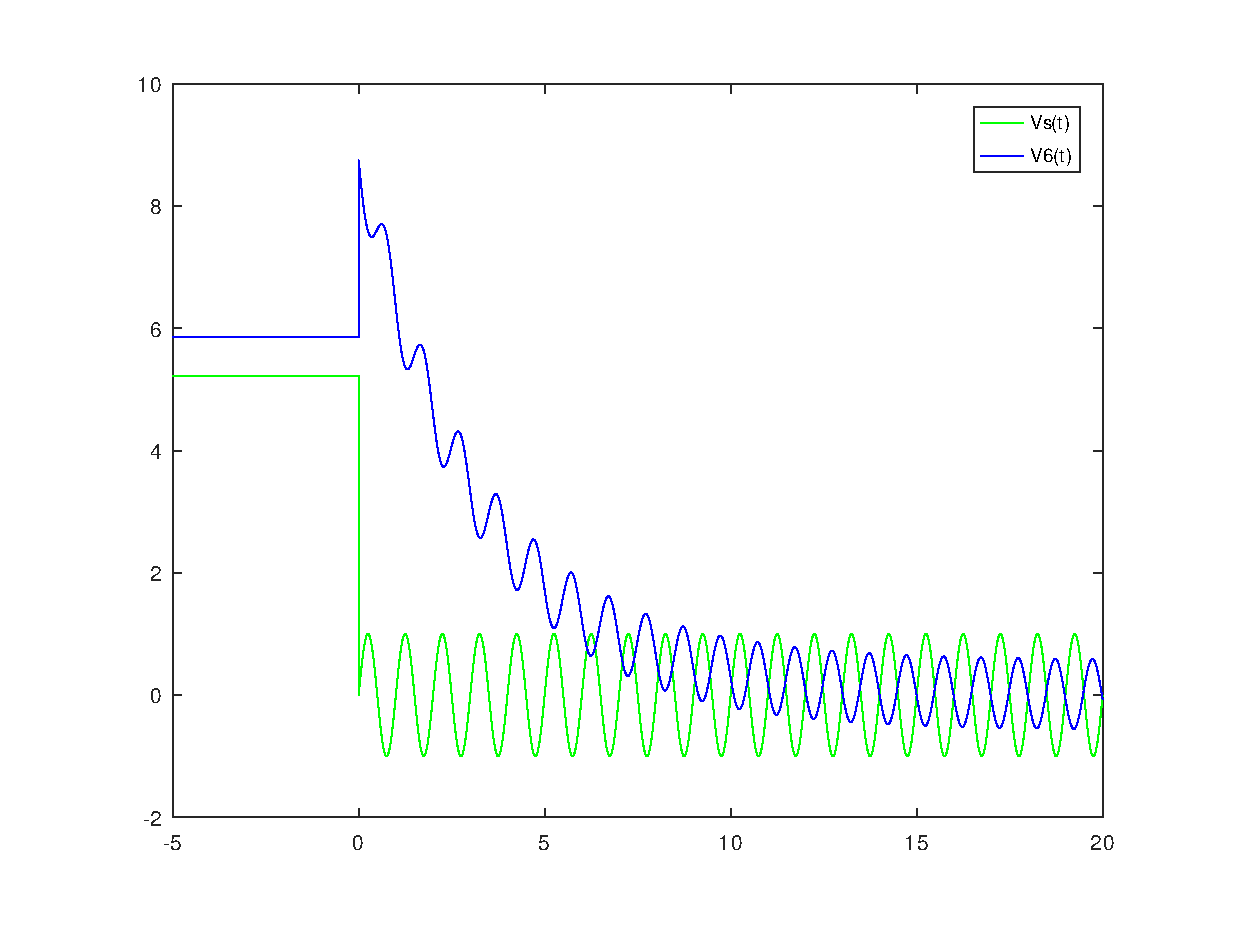
\includegraphics[width = 8cm]{Solution.eps}
\caption {Natural and forced response}
\end{figure}


\subsection{Point 6: Determine the frequency response for Vc(f), V6(f) and Vs(f)}

In the final section of the work we just needed to repeat the point 4 multiples times modifying the fequencies of the source, to see how the amplitude and phase of Vc(f) (that is V6 - V8), V6(f) and Vs(f). The results can be seen below.

\begin{figure}[H]
\centering
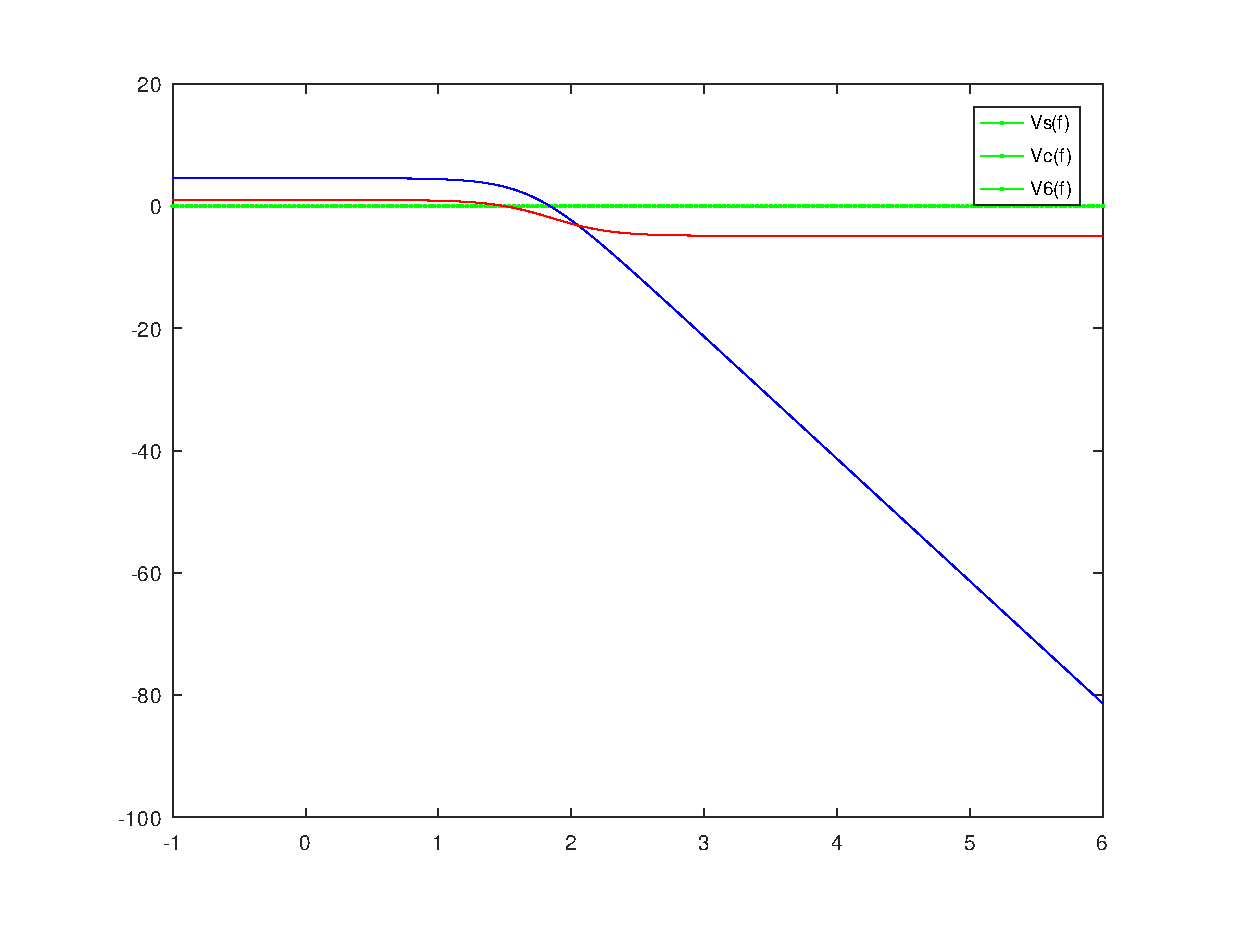
\includegraphics[width = 8cm]{Amplitude.eps}
\caption {Amplitude}
\end{figure}

\begin{figure}[H]
\centering
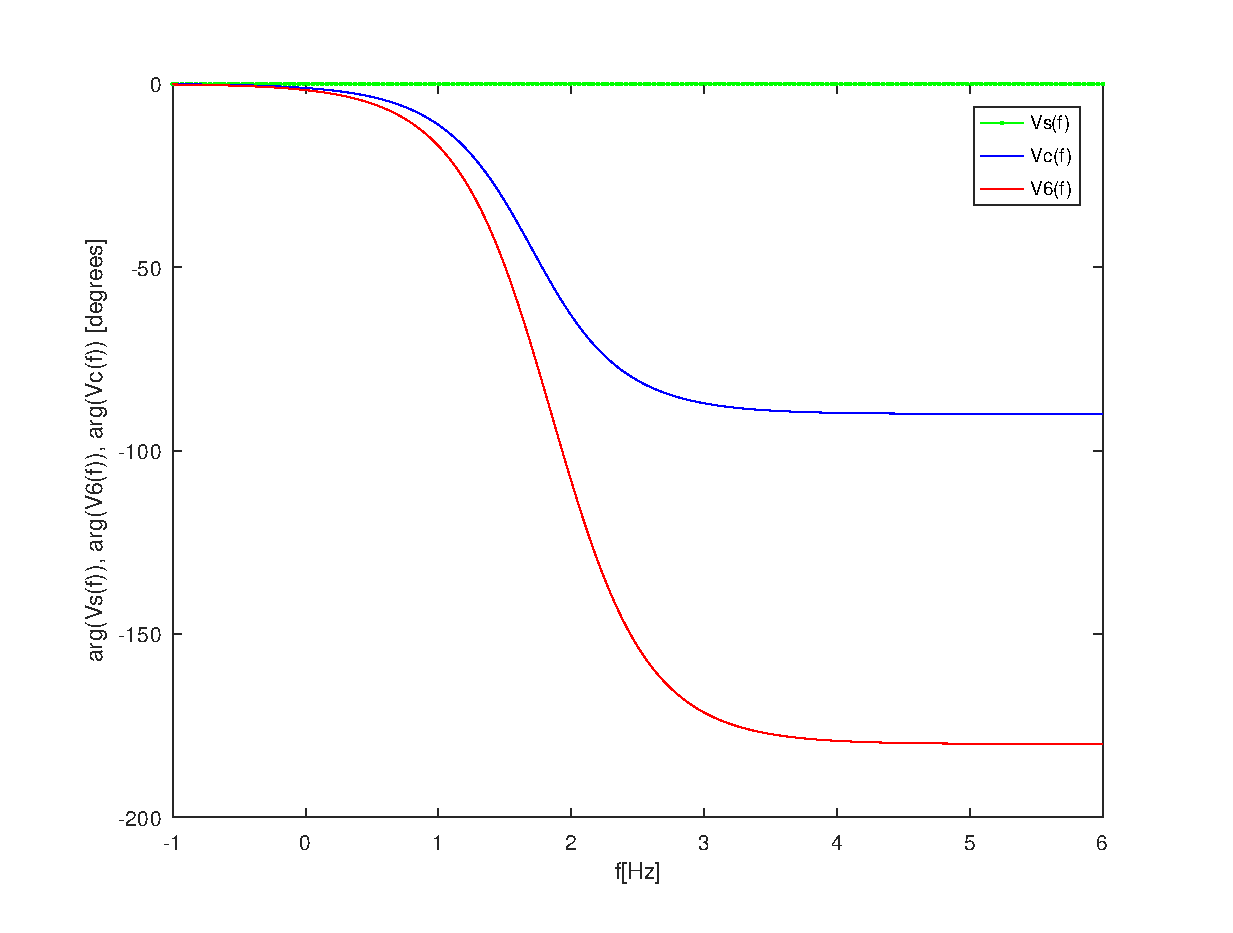
\includegraphics[width = 8cm]{Arguments.eps}
\caption {Arguments}
\end{figure}
